% ============================================================
% CAPÍTULO 1: INTRODUCCIÓN
% ============================================================

\chapter{Introducción}
\label{chap:introduccion}

\subsection{Fundamentos de la Electrocardiografía (ECG)}

Un electrocardiograma (ECG) es una representación gráfica de la actividad eleéctrica del corazón en función
del tiempo. Debido a que en cada latido se produce una despolarización y una repolarización de las células,
se generan potenciales eéctricos que pueden ser detectados desde la superficie del cuerpo.

Para capturar esta señal, se colocan electrodos sobre la superficie del cuerpo del paciente, en puntos
específicos, capaces de medir la diferencia de potencial eléctrico generada por este latido. 

La combinación de estos electrodos da lugar a las \textit{derivaciones}. En la práctica,
se suele utilizar el sistema de 12 derivaciones, el cual se divide en:
\begin{itemize}
    \item \textbf{Derivaciones bipolares (I, II, III):} Miden la diferencia de potencial
    entre dos extremidades (siguiendo el triángulo de Einthoven).
    \item \textbf{Derivaciones monopolares aumentadas (aVR, aVL, aVF):} Miden el potencial
    en una extremidad respecto a un punto de referencia central.
    \item \textbf{Derivaciones precordiales (V1 a V6):} Situadas directamente sobre el tórax para
    observar la actividad eléctrica en el plano horizontal del corazón.
\end{itemize}

\begin{figure}[htbp]
  \centering
  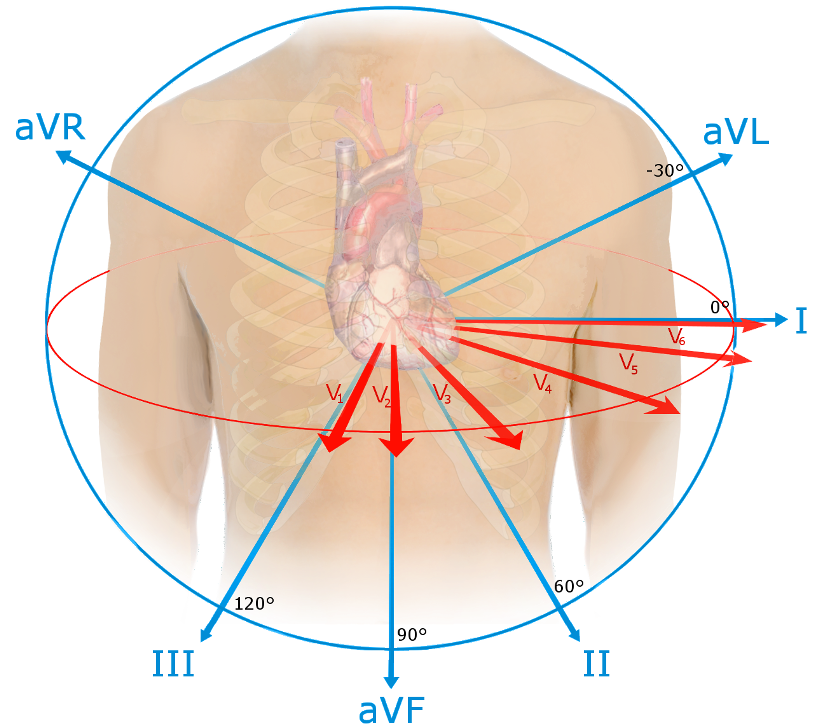
\includegraphics[width=0.5\textwidth]{img/EKG_leads.png}
  \caption{Orientación espacial de las derivaciones ECG. Imagen obtenida de \href{https://en.wikipedia.org/wiki/Electrocardiography}{Wikipedia}.}
  \label{fig:orientacion_derivaciones}
\end{figure}

Cada derivación observa el mismo fenómeno eléctrico, pero desde un ángulo espacial distinto. Esto resulta
clave para la detección de patologías como arritmias o infartos. \cite{wikipedia_electrocardiography_2026}

% ---------- cambiar si hay timepo hacia arriba

La Fibrilación Auricular (FA) es la arritmia cardíaca más común, caracterizada por un comportamiento
auricular caótico (como se ilustra en la Figura~\ref{fig:ejemplo}).
Esta patología provoca una pérdida de la contracción auricular efectiva, lo que incrementa
el riesgo de formación de trombos, accidentes cerebrovasculares (ictus), insuficiencia cardíaca
y deterioro cognitivo a largo plazo \cite{wikipedia_atrial_2026}.

\begin{figure}[htbp]
  \centering
  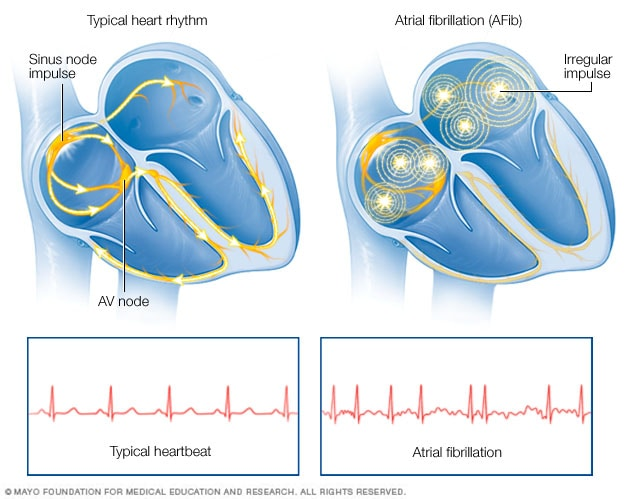
\includegraphics[width=0.7\textwidth]{img/atrial fibrilation.jpg}
  \caption{Ejemplo de ECG en fibrilación auricular. Imagen obtenida de la \href{https://www.mayoclinic.org/diseases-conditions/atrial-fibrillation/symptoms-causes/syc-20350624}{Mayo Clinic}.}
  \label{fig:ejemplo}
\end{figure}

Dentro de sus varaintes, se encuentra la Fibrilación Auricular Paroxística (PAF, por sus siglas en
inglés, \textit{Paroxysmal Atrial Fibrillation}). Ésta se caracteriza por episodios esporádicos de arritmia,
que se inician de manera espontánea y que vuelven al ritmo sinusal en un periodo de unos 7 días, aunque la mayoría lo hacen en menos de 24 horas.

Debido a esta naturaleza intermitente, los ECGs de corta duración no suelen capturarlos. Por ello, la predicción inminente de estos episodios, 
es decir, tener la capacidad de predecir si un paciente sufrirá un episodio en los próximos
minutos a partir de su ritmo sinusal, en holters de larga duración es de especial interés.

Predecir un episodio con una ventana de antelación de hasta 5 minutos permitiría alertar al paciente para que cese
actividades de riesgo, automatizar la administración preventiva de fármacos
antiarrítmicos o preparar dispositivos de estimulación eléctrica cardíaca adaptativa.

Sin embargo, la predicción es una tarea compleja. La fase previa al episodio arrítmico es en ritmo sinusal,
por lo que a simple vista en el ECG no se observan patrones o anomalías morfológicas evidentes.

\section{Contexto del Trabajo}
\label{sec:contexto}

Clasicamente este problema solia abordarse mediante la extracción de características de
variabilidad del ritmo cardíaco (HRV, \textit{Heart Rate Variability}) y por un clasificador lineal. Sin embargo esta
estrategia no suele ser capaz de analizar las distorsiones morfológicas locales de las señales
de ECG (como cambios finos en la onda P o en el intervalo PR) que preceden a la FA.

Las redes neuronales cambian la forma de abordar este problema, permitiendo extraer información
directamente de la señal ECG sin procesar. No obstante hay que tener en cuenta algunas limitaciones
como:

\begin{enumerate}
  \item \textbf{Sesgo de Base de Datos:} Se entrenan utilizando una única base
  de datos. Esto genera modelos altamente sobreajustados a las condiciones de ruido y
  hardware de esa base de datos concreta, que fracasan al ser validados en registros
  independientes.
  \item \textbf{Data Leakage y validaciones débiles:} Con frecuencia se comparten
  ventanas del mismo paciente entre los conjuntos de entrenamiento y test,
  reportando precisiones artificialmente altas.
\end{enumerate}

Este trabajo se enfoca en resolver estas limitaciones utilizando un dataset
procedente de distintas bases de datos, evaluando los modelos mediante una validación cruzada inter-sujeto.


\section{Objetivos del Proyecto}
\label{sec:objetivos}

El objetivo de este proyecto es
\textbf{diseñar, implementar y evaluar un sistema capaz de
predecir de forma inminente (en una ventana de 5 minutos antes del inicio) episodios de
Fibrilación Auricular Paroxística (PAF) a partir de segmentos de 1 minuto de señal ECG en
ritmo sinusal}.

Para alcanzar este fin, se definen los siguientes objetivos:
\begin{itemize}
  \item \textbf{Objetivo 1:} 
  Integrar cinco bases de datos heterogéneas de PhysioNet:
  \textit{afpdb}, \textit{cpsc2021}, \textit{ltafdb}, \textit{shdb-af} y \textit{afdb}.
  \item \textbf{Objetivo 2:} 
  Desarrollar un pipeline de preprocesamiento que permita la
  extracción de ventanas variables de ritmo sinusal Pre-PAF y de características
  temporales y frecuenciales de HRV.
  \item \textbf{Objetivo 3:} 
  Entrenar distintas arquitecturas de redes neuronales como: ResNet 1D (modelo base residual),
  SEResNet 1D (con atención por canal Squeeze-and-Excitation),
  un modelo CNN-Transformer (\textit{multi-head self attention})
  y Mamba 1D (basado en \textit{state space models}).
  \item \textbf{Objetivo 4:} 
  Integrar la información de HRV mediante una cabeza clasificatoria
  (Multi-Layer Perceptron) que potencie la toma de decisiones de
  las redes.
  \item \textbf{Objetivo 5:} 
  Evaluar rigurosamente los modelos bajo un diseño GroupKFold para mitigar
  la filtración de datos.
\end{itemize}


